\chapter{Make Distinct}

\section{Experiment Setup}

The setup for this experiment is quite simple. The data types tested on in this experiments are:
\mintinline{rust}{i32}, a slightly modified \mintinline{rust}{f64}, \mintinline{rust}{String}, and mixed records. 
For the purpose of this experiment, the mixed record is called \mintinline{rust}{Cat}. The details for this will be brought up later on.
As for the size of the input, the sizes used are $10^2, 10^4, 10^5, 10^6$, and $10^7$. I can probably go higher but \textit{I don't want my computer to fly off my desk yet when testing with even larger inputs.}

The functions for de-duplication are implemented according to the handout. Note that in both implementation, the input vector is duplicated first so that the input itself doesn't get modified.
\begin{itemize}
\item \mintinline{rust}{unique_hashset} creates a hash-based set from the input vector then creates the final vector from the set's iterator
\item \mintinline{rust}{unique_sorted} sorts the input vector then pushes an element into the resulting vector every time a pair of adjacent elements are different
\end{itemize}

\subsection*{Fraction of Repetition (FoR)}

In order to investigate the effects of the FoR on the running time, we want to be able to specify it in each run of the experiment.
So, for each size $n$ of the input vector, we compute the number of distinct elements needed for the input vector to have a certain FoR and randomly generate a vector of distinct elements. Then, to create the input vector, we randomly pick from the distinct vectors until we get the input size that we want.

The specified FoRs used for this experiments are $0.1, 0.25, 0.5$, and $0.75$ but the highest FoR I was able to actually achieve was around 0.6 for this experiment. This could be due to the RNG engine used but I did not look further into it.

\subsection*{Dealing with Floating-point Numbers}

As mentioned to me by Aj. Kanat while I was working on this problem in 1502, \textit{you cannot sort floats!}
This is because \mintinline{rust}{f64}s are not ordered nor hash-able. So, we need to find a way to solve these issues.
The solution that I came up with is to use a wrapper for \mintinline{rust}{f64} called \mintinline{rust}{F64} and implementing \mintinline{rust}{Ordering} and \mintinline{rust}{Hash}.

For the ordering, a simple comparator is created for floats--subtract and see the sign of the sum then return accordingly.
This is still subject to the problem of rounding error, but for the sake of my sanity, \textit{I will assume that this is enough}.
For the hashing, this was done by separating the bit representation into 3 parts: sign, exponent, and Mantissa using some (evil/unsafe) bit tricks.
Then, form a \mintinline{rust}{[u64; 3]} from these three and hashing them since this has become a problem of hashing an array of integers.

Obviously, this solution is far from perfect but, eh, \textit{I will assume that this is enough to save my sanity.}

\subsection*{Dealing with Mixed Records}

As mentioned before, the mixed record here is called \mintinline{rust}{Cat} for \textit{obvious reasons--cats just make your life (mostly) better.} (I don't own one. Sad.) It is comprised of a string for name, an integer for age, a floating-point number for weight, and a collection of unsigned integers for the phone number of its owners with a maximum size of 5. Specifically, a \mintinline{rust}{Cat} is defined as the following.

\begin{minted}{rust}
#[derive(Hash, Clone)]
pub struct Cat {
    name: String,
    age: u8,
    weight: F64,
    owner_phone_numbers: Vec<u32>,
}
\end{minted}

Since every member of \mintinline{rust}{Cat} is hash-able, the implementation for \mintinline{rust}{Hash} is derived.
However, the ordering needs to be implemented. So, the ordering is defined as the following. A cat $A$ is \textit{less} than cat $B$ when $A$'s age is less than $B$'s. If they are of the same age, $A$ would weight less. If they also weight the same, their names will be compared lexicographically. If all of above are equal, then they are the same cat. \textit{The tracker just forgot to update the phone numbers of their owners}.
Why? I don't know. I just came up with this scheme on a whim.

\section{(Quick) Time and Space Analysis}

\subsection*{Hash-based Set}

The function that de-duplicates the input does the following. First, it clones the input array, taking $O(n)$ time.
Then, assuming the hash function for each data type takes constant time, it creates a hash set from the cloned input array, taking $O(n)$.
Finally, it creates a new vector from iterating over the set, taking $O(n)$. Therefore, the asymptotic running time of this function is $O(n)$. However, this running time could also be affected by the running time of the hash function.

During the de-duplication of an input vector with length $n$, 2 new vectors of maximum length $n$ are created along with a hash set of maximum size $n$. Thus, the space requirement of this function is $O(n)$.

\subsection*{Sorting}

The function that de-duplicates the input does the following. First, it clones the input array, taking $O(n)$ time.
Then, it sorts the cloned array, taking $O(n \log n)$ as mentioned in Rust's documentation.
Finally, it creates a new vector from iterating over the sorted vector, taking $O(n)$. Therefore, the asymptotic running time of this function is $O(n \log n)$ which is asymptotically slower than using the hash set. This could also be made worse depending on the comparator as well.

During the de-duplication of an input vector with length $n$, 1 new vector of length $n$ is created as a clone. Then, Rust's implementation of sorting could create a temporary slice of size at most $n/2 \in O(n)$. Finally, it creates the returning array. Therefore, the space requirement for this is $O(n)$ but the constant would be less than the hash-based implementation.

\newpage

\section{Results}
\begin{figure}[h]
	\centering
	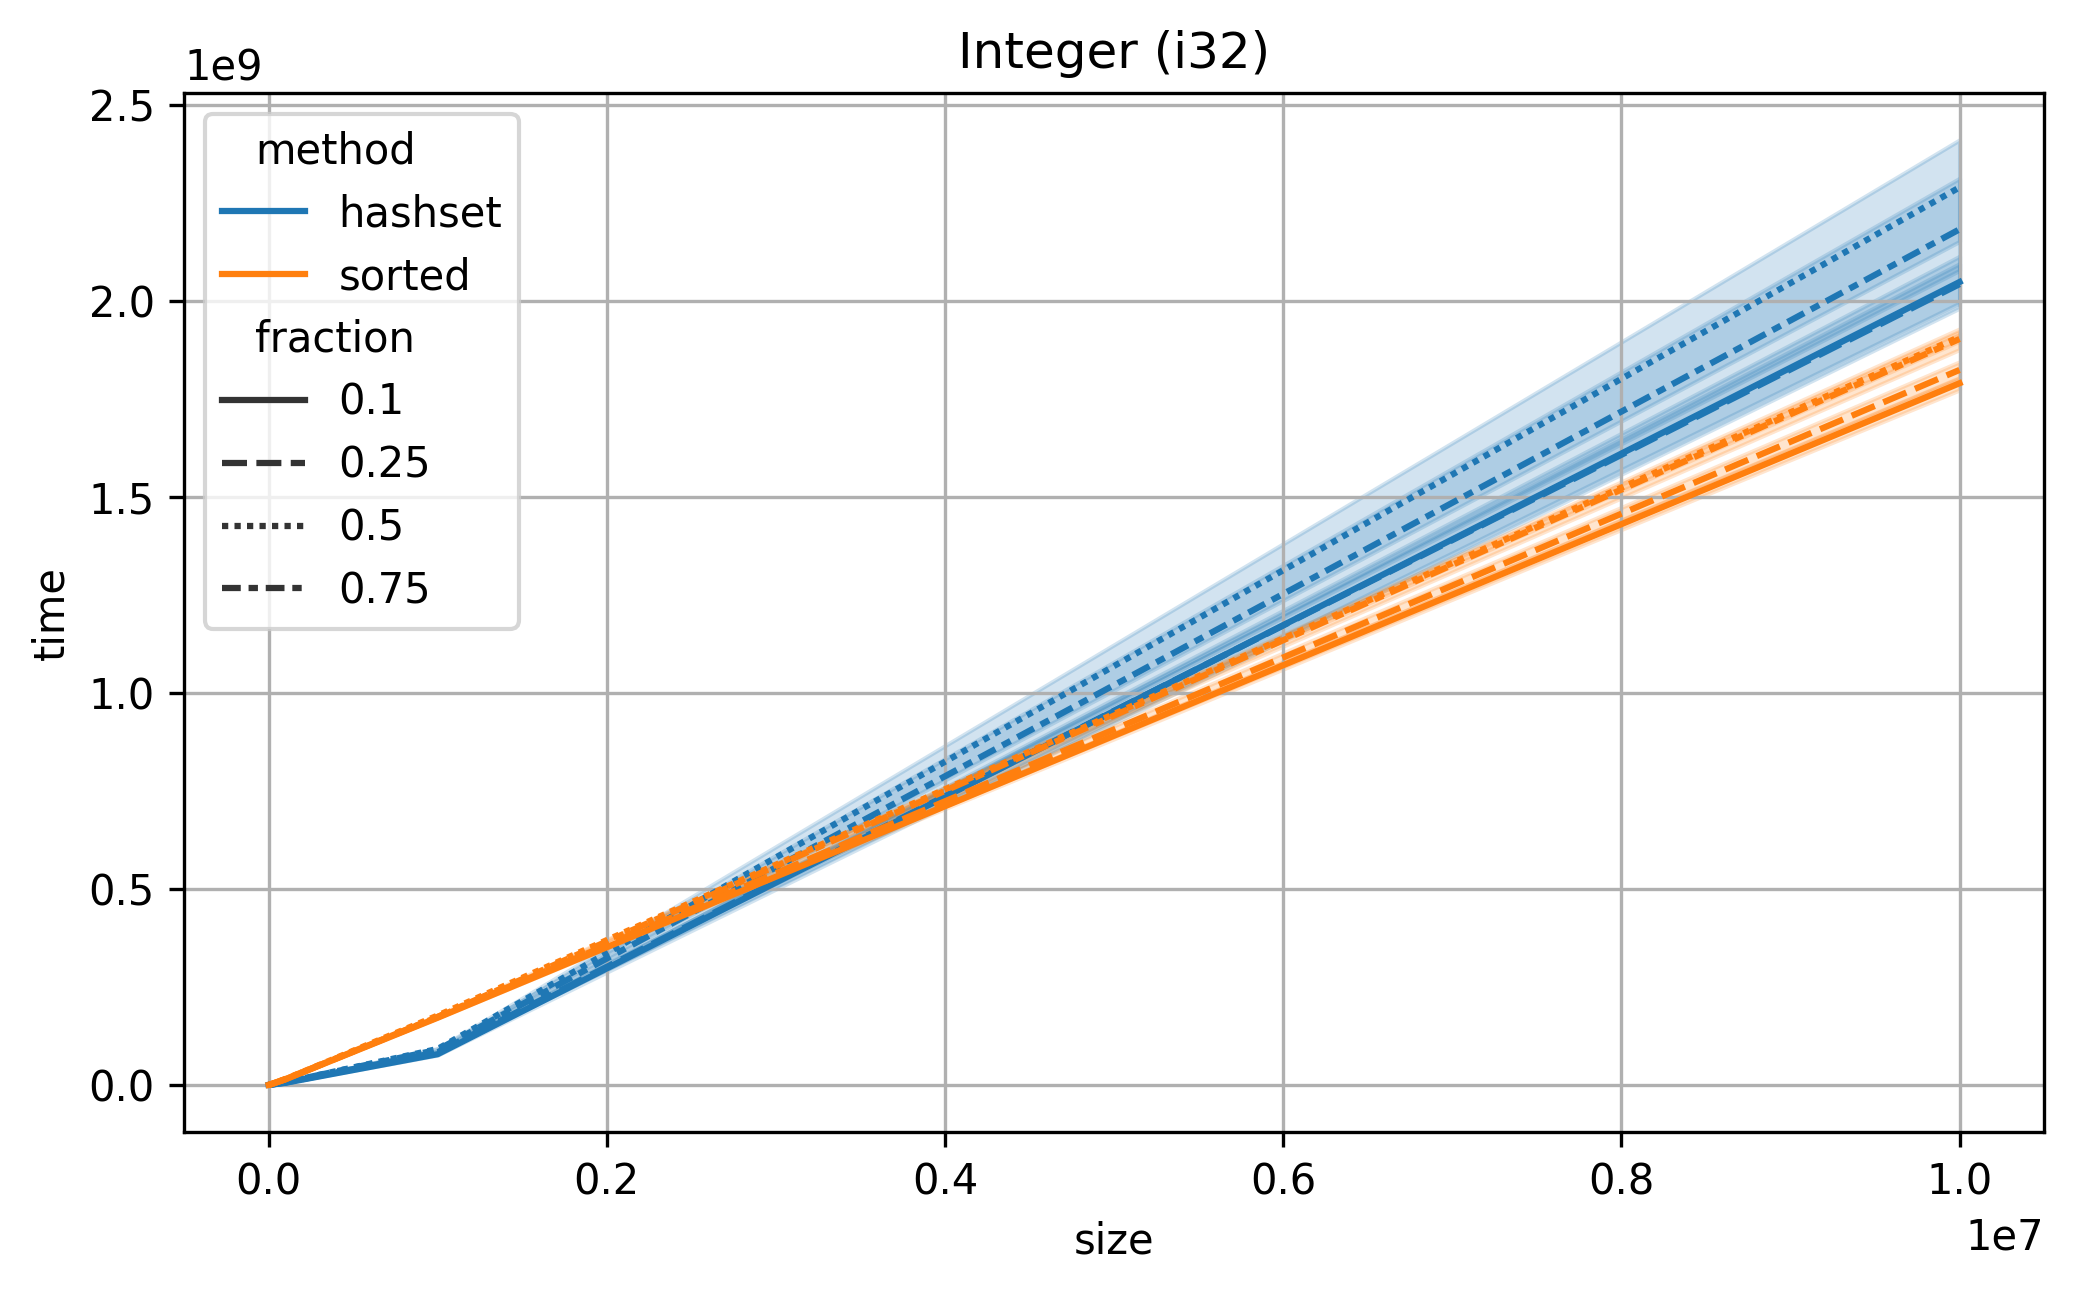
\includegraphics[width=0.8\textwidth]{graphics/03-int.png}
	\caption{Number of cycles taken for de-duplication of a vector of integers}
\end{figure}

\begin{figure}[h]
	\centering
	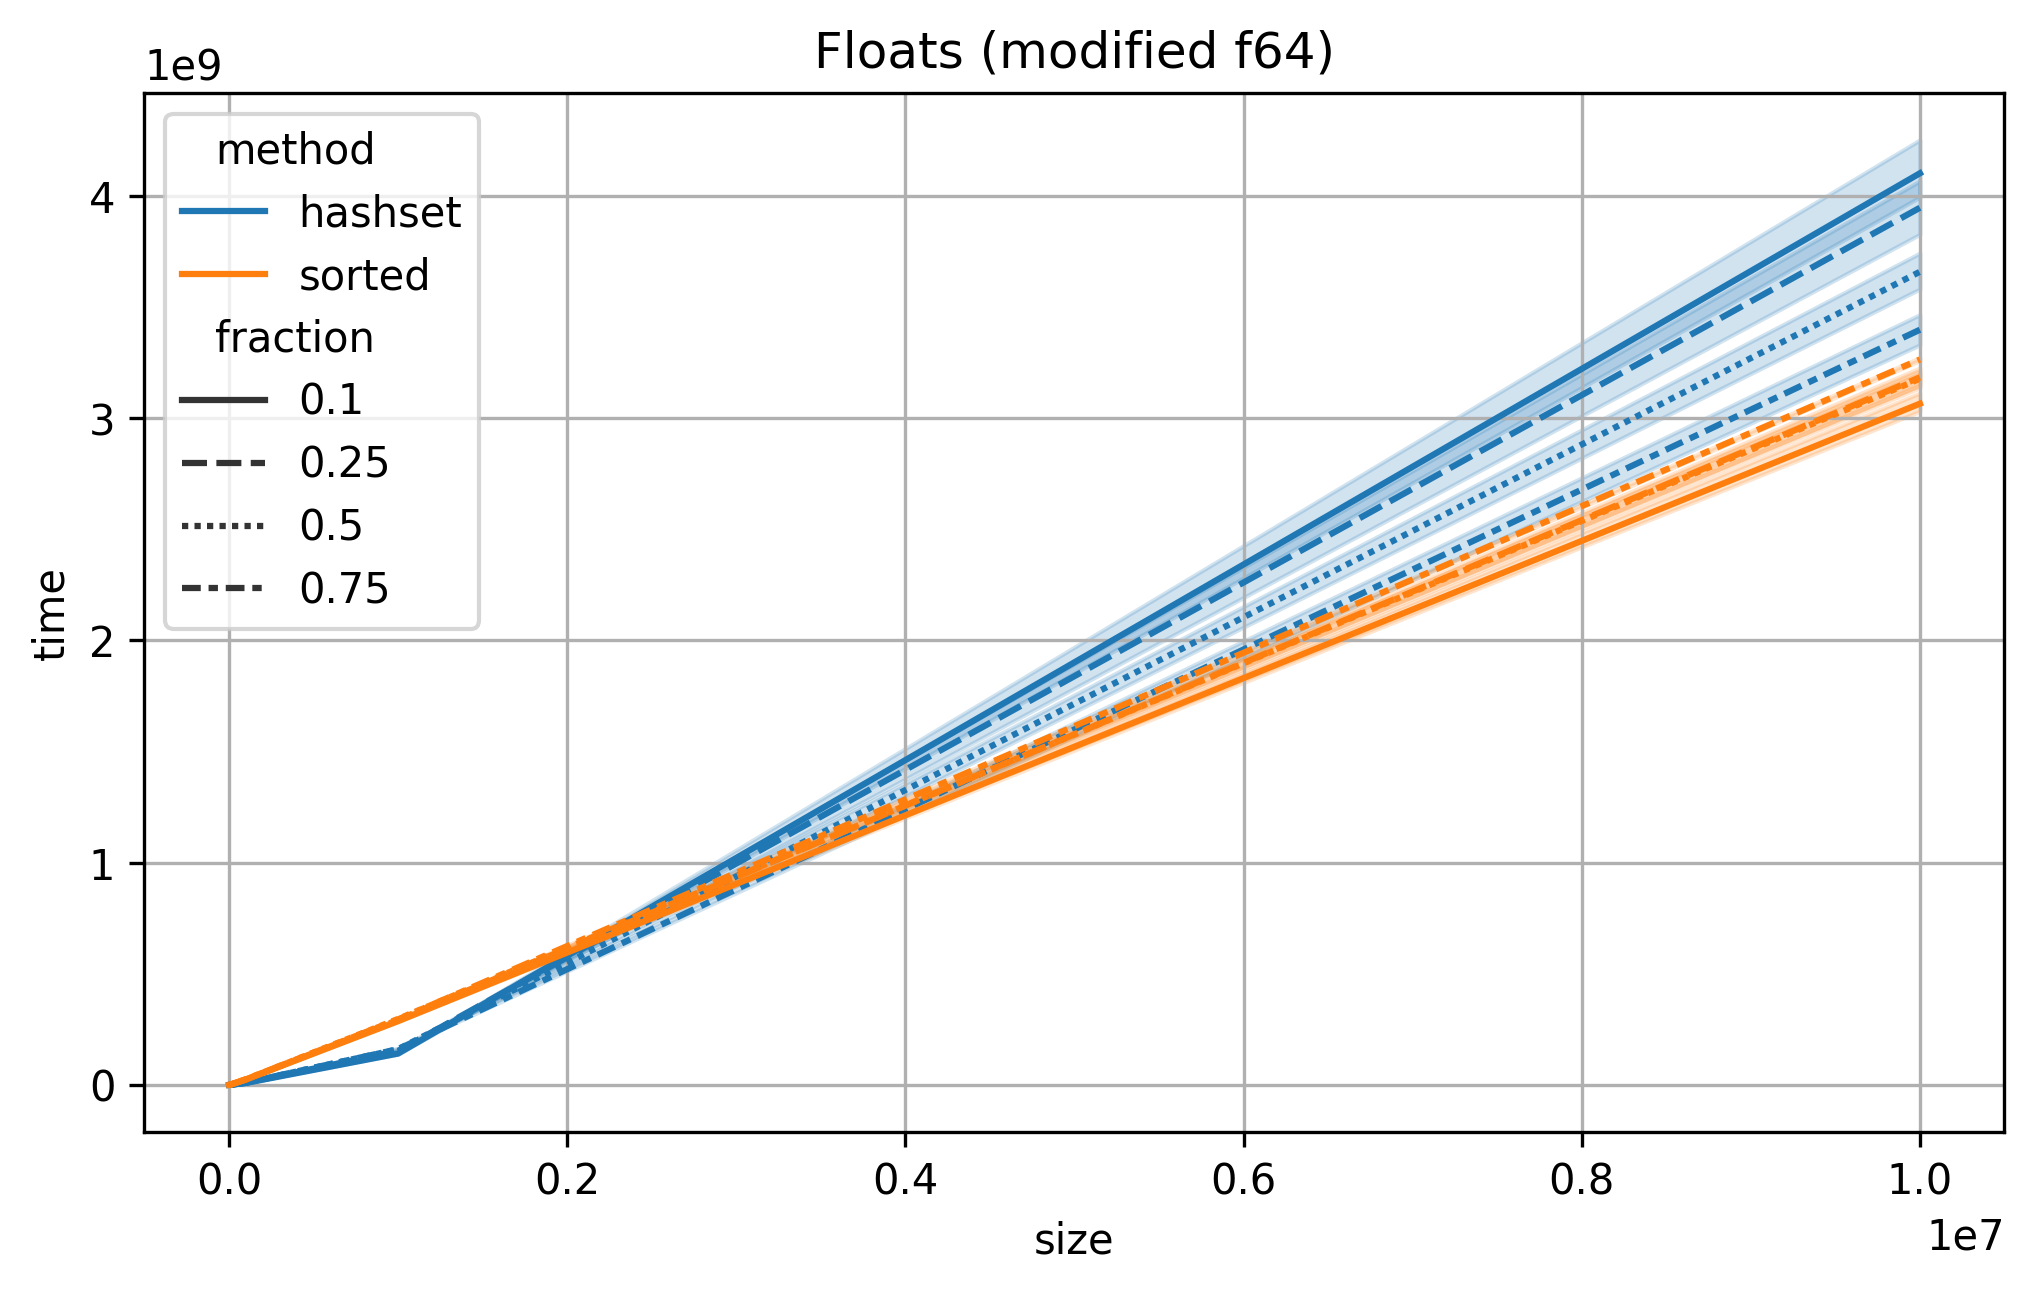
\includegraphics[width=0.8\textwidth]{graphics/03-float.png}
	\caption{Number of cycles taken for de-duplication of a vector of floats}
\end{figure}

\newpage

\begin{figure}[h]
	\centering
	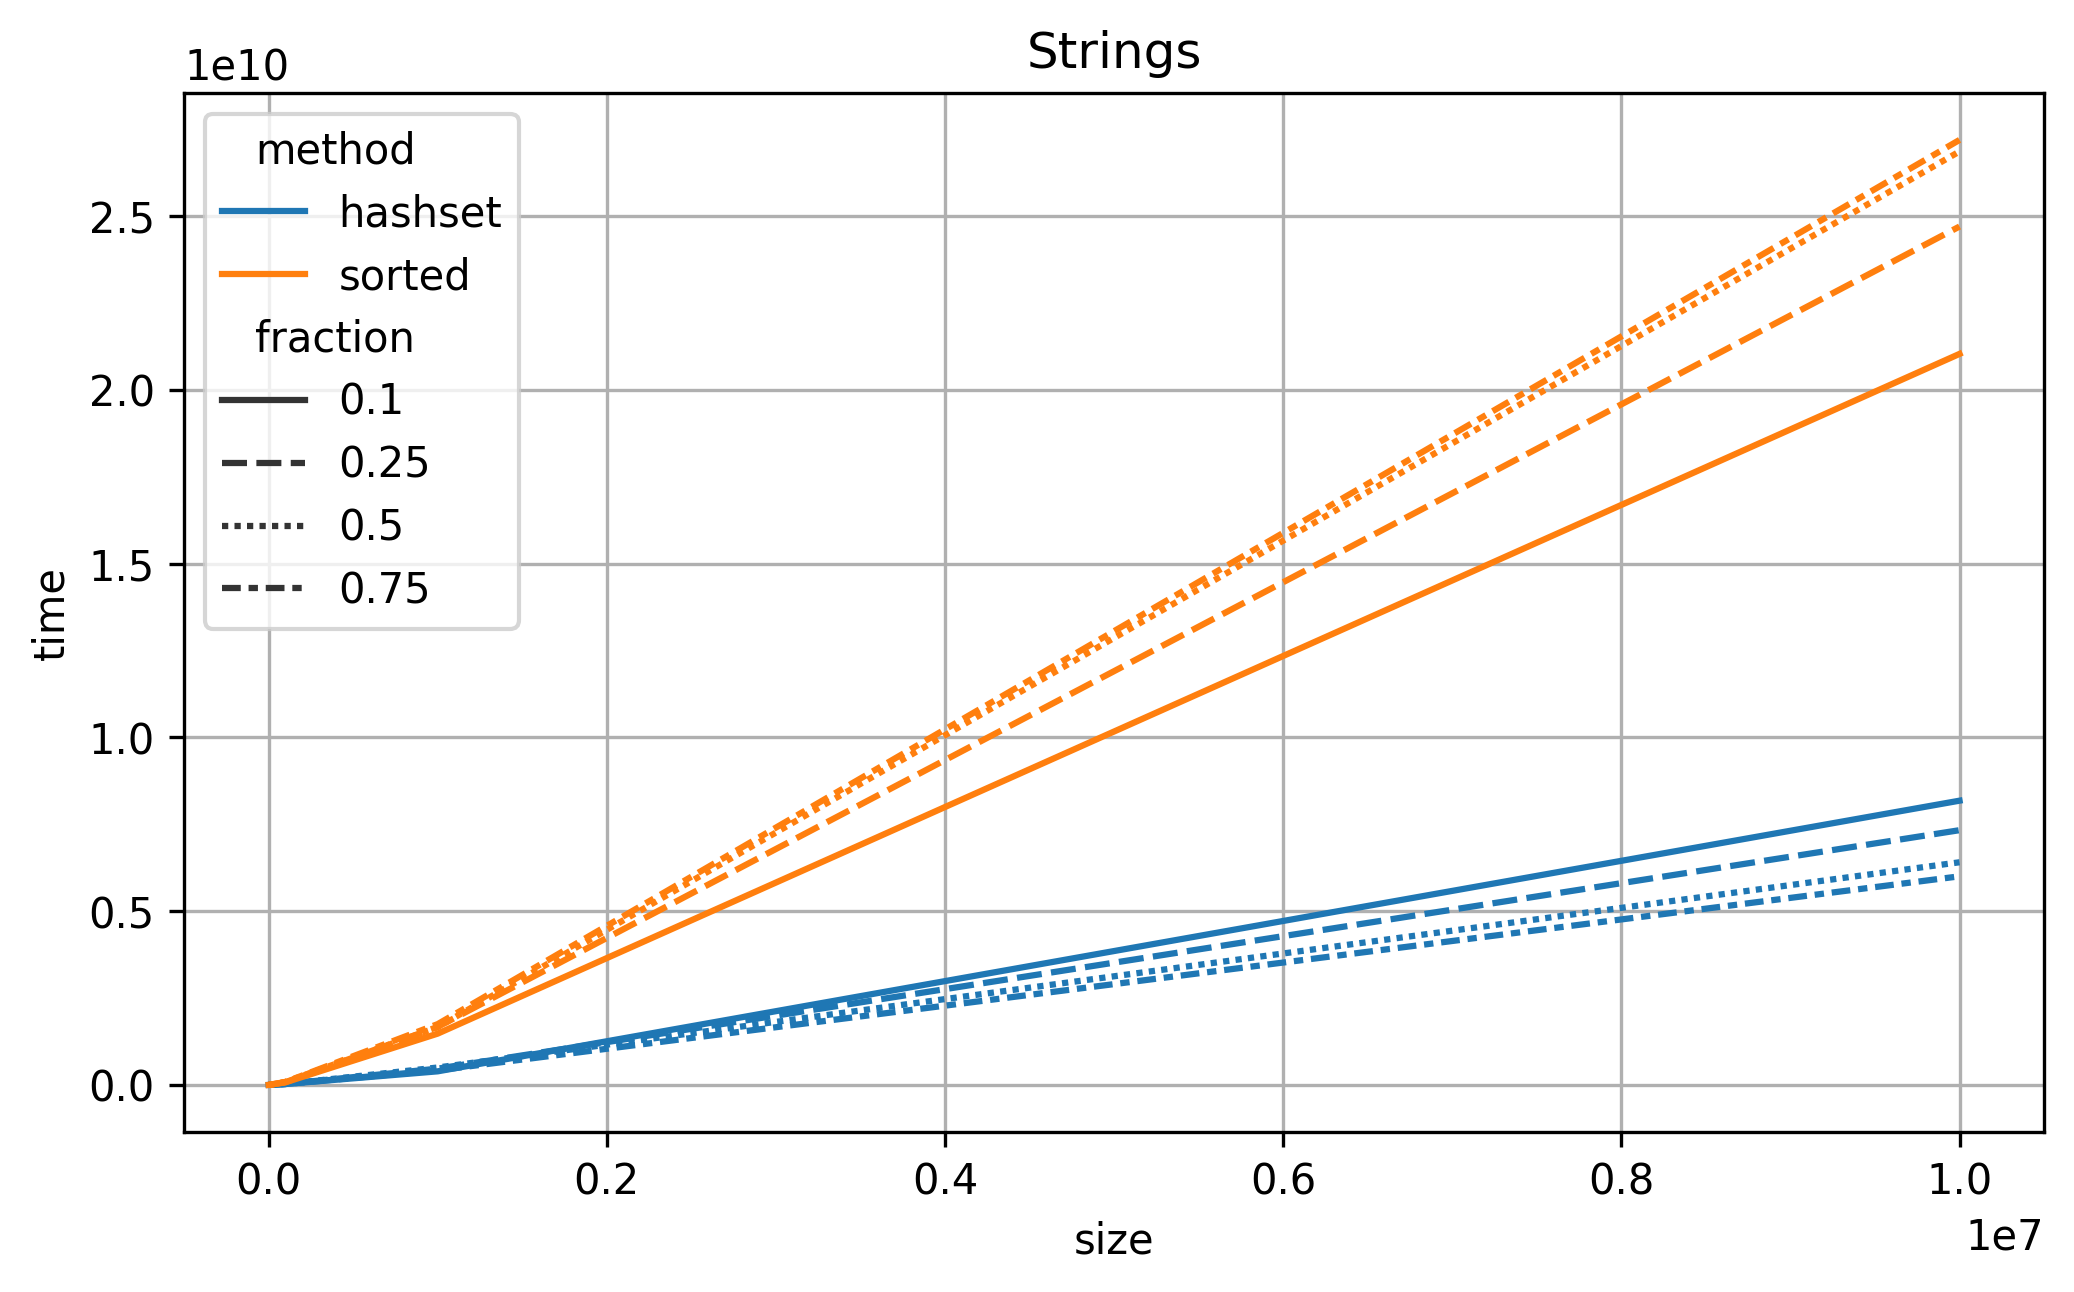
\includegraphics[width=0.8\textwidth]{graphics/03-string.png}
	\caption{Number of cycles taken for de-duplication of a vector of strings}
\end{figure}

\begin{figure}[h]
	\centering
	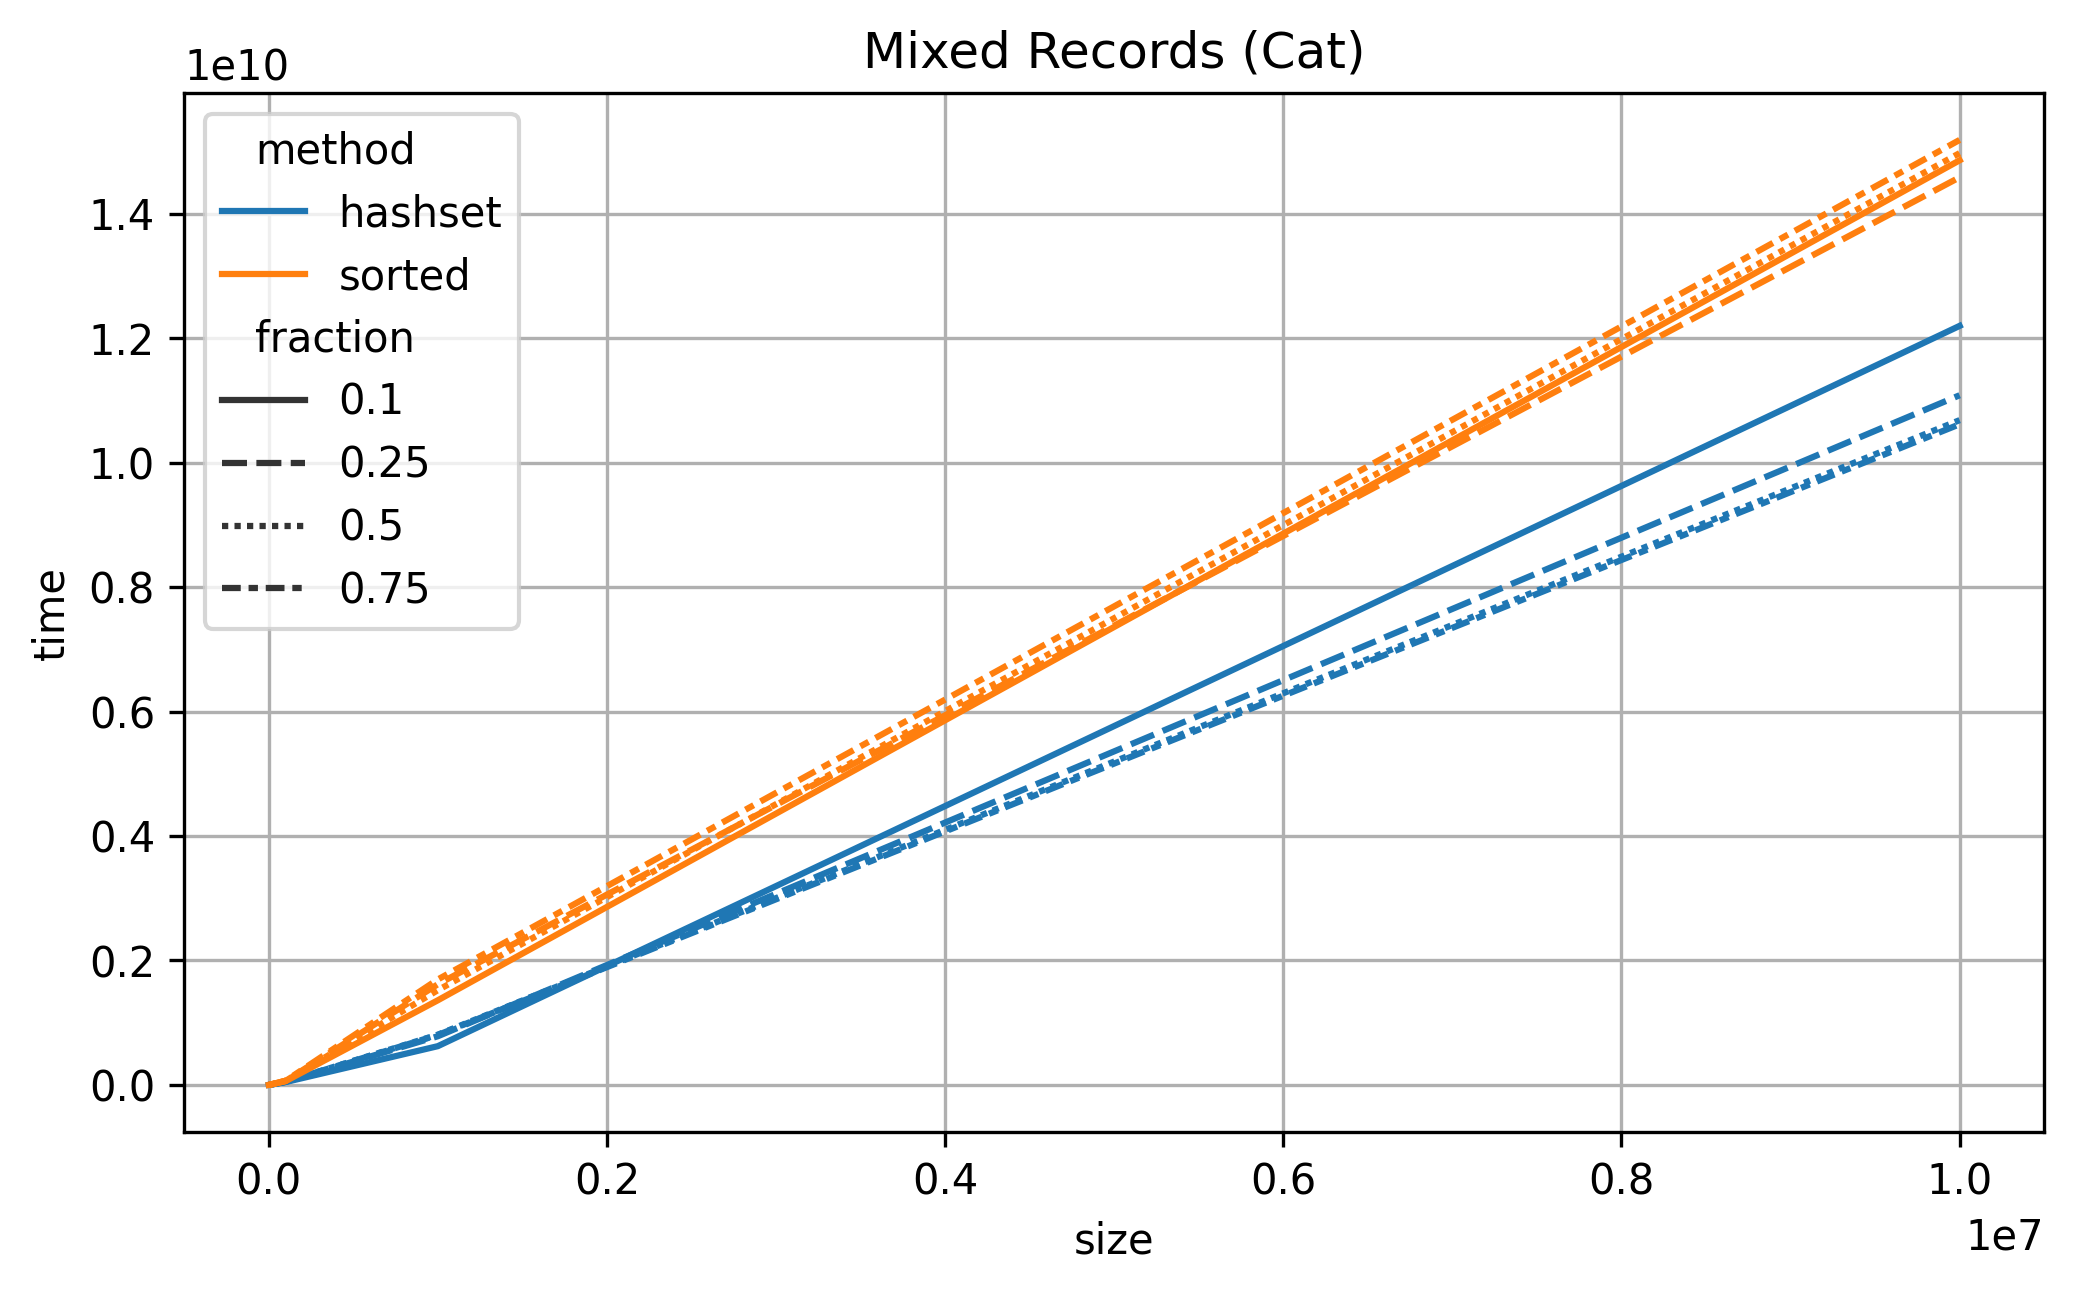
\includegraphics[width=0.8\textwidth]{graphics/03-cat.png}
	\caption{Number of cycles taken for de-duplication of a vector of mixed records}
\end{figure}

\section{Conclusion}

It seems that, for simple, fixed-sized data types that are (somewhat) ordered, sorting is the way to go. This could be because the simpler comparisons take significantly less time than computing the hash. This could also be due to its relatively smaller size so more elements can fit in a single cache line which leads to faster access latency when sorting and accessing neighboring elements.

In contrast, strings and mixed records are clearly faster with hashing. In this case, sorting could be slower because string comparison is proportional to its length and the mixed records' larger size could decrease cache hits, adding latency to access time during sorting while hashing is relatively constant time for all elements and adding to a set is similar as well.
Its variable length could also be another factor but I have no real reasoning for this. My guess is that in order to sort variable-length data, there could be some \textit{buffer space} per element so any large element could fit anywhere when put in the resulting collection which, again, adds access latency.

Interestingly, FoRs have a big impact with the hash-based implementation where the more duplicates there are, the slower it runs. Sorting-based implementation seems to be unaffected by FoRs except for strings but the number of cycles seems to be around the same in other cases.

In conclusion, the better method depends on the use case. However, with databases usually being comprised of mostly mixed records, hashing may be the way to go assuming that that database is not indexed/already ordered in some way.
